\documentclass{beamer}

\usepackage{amsmath}
\usefonttheme{serif}

\usepackage{ctex} 
\usepackage{amsmath}
\usepackage{amsfonts}
\usepackage{minted}
\usepackage{graphics}
\usepackage{booktabs}
\usepackage{xeCJK}
\setCJKmainfont[ItalicFont={楷体}, BoldFont={黑体}]{宋体}

\usepackage{booktabs}

\newcommand{\E}{\text{E}}
\newcommand{\var}{\text{Var}}
\newcommand{\cov}{\text{Cov}}
\renewcommand{\d}{\text{d}}

\setbeamertemplate{footline}[frame number]

\title{为 rCore 实现更多系统调用}

\author{罗崚骁 \quad 宋香君}

\begin{document}
\begin{frame}
    \titlepage
\end{frame}

\begin{frame}{课程设计目标}
    \begin{itemize}
        \setlength{\itemsep}{10pt}
        \item rCore 自编译
        \begin{itemize}
            \setlength{\itemsep}{10pt}
            \item musl-libc 完善
            \item Make, CMake
            \item Rustc, Cargo
            \item 文件系统支持
        \end{itemize}
    \end{itemize}
\end{frame}

\begin{frame}{目前进展}
    {运行 shell 脚本}
    \begin{itemize}
        \setlength{\itemsep}{10pt}
        \item ash + 脚本文件名运行脚本(sys\_dup,fcntl)
        \item 命令替换(Command Substitution)
        \begin{itemize}
        \setlength{\itemsep}{10pt}
            \item 诸如 echo \$(echo 233) 这样的命令
            \item 需要对管道增加阻塞
        \end{itemize}
        \item 可以跑通 make 的 configure 脚本和构建脚本
    \end{itemize}
\end{frame}

\begin{frame}{目前进展}
    {GNU Make}
    \begin{itemize}
        \setlength{\itemsep}{10pt}
        \item 能够在 rCore 内部缺少 make 的情况下构建,configure+build.sh
        \item 基本功能正常运行,可以使用 3.78.1 的 make 构建出3.79 的 make
        \item 支持增量构建
        \begin{itemize}
            \item 增加了文件系统对修改时间的记录,完善了对 stat 的实现,顺便还能支持 touch
        \end{itemize}
    \end{itemize}
\end{frame}

\begin{frame}{目前进展}
    {libc-test}
    \begin{itemize}
        \setlength{\itemsep}{10pt}
        \item Makefile 正常执行
        \item 给出了所有测例的执行结果
        \begin{itemize}
            \setlength{\itemsep}{10pt}
            \item 258 个测例成功
            \item 215 个测例失败,其中 18 个测例无法正常结束
            \item 失败的测例主要是 pthread(缺少信号机制支持)、math(大量计算错误,140 个左右) 相关
            \item 修好了全部信号量相关的测例
        \end{itemize}
    \end{itemize}
\end{frame}

\begin{frame}{后续任务}
    {Cargo}
    \begin{itemize}
        \setlength{\itemsep}{10pt}
        \item 目前只能新建项目,还无法成功使用 Cargo 构建
        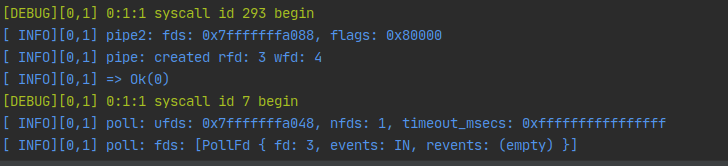
\includegraphics[width=\linewidth]{assets/cargo.png}
        \begin{figure}[htbp]
            \centering
            % \caption{}
            % \label{}
        \end{figure}
    \end{itemize}
\end{frame}

\begin{frame}{后续任务}
    {libc-test}
    \begin{itemize}
        \setlength{\itemsep}{10pt}
        \item 主要针对 pthread 和数学的相关测例进行修复
        \item 增加信号机制,实现一些和信号相关的系统调用
        \item 编写文档,总结 rCore 开发微小的经验
    \end{itemize}
\end{frame}

\begin{frame}{调试方法}
    \begin{itemize}
        \setlength{\itemsep}{10pt}
        \item 除了可以开启记录模式打印每条系统调用外,还可以用 gdb 通过
        相应端口连接到 qemu 进行调试
        \item 使用 CLion 提供的 gdb remote debug 可以在 IDE 中更方便地定位到错误
        \item 不过目前 rCore 的 Debug 版也开了 O2,调试时困难变大
    \end{itemize}
\end{frame}

\begin{frame}{调试方法}
    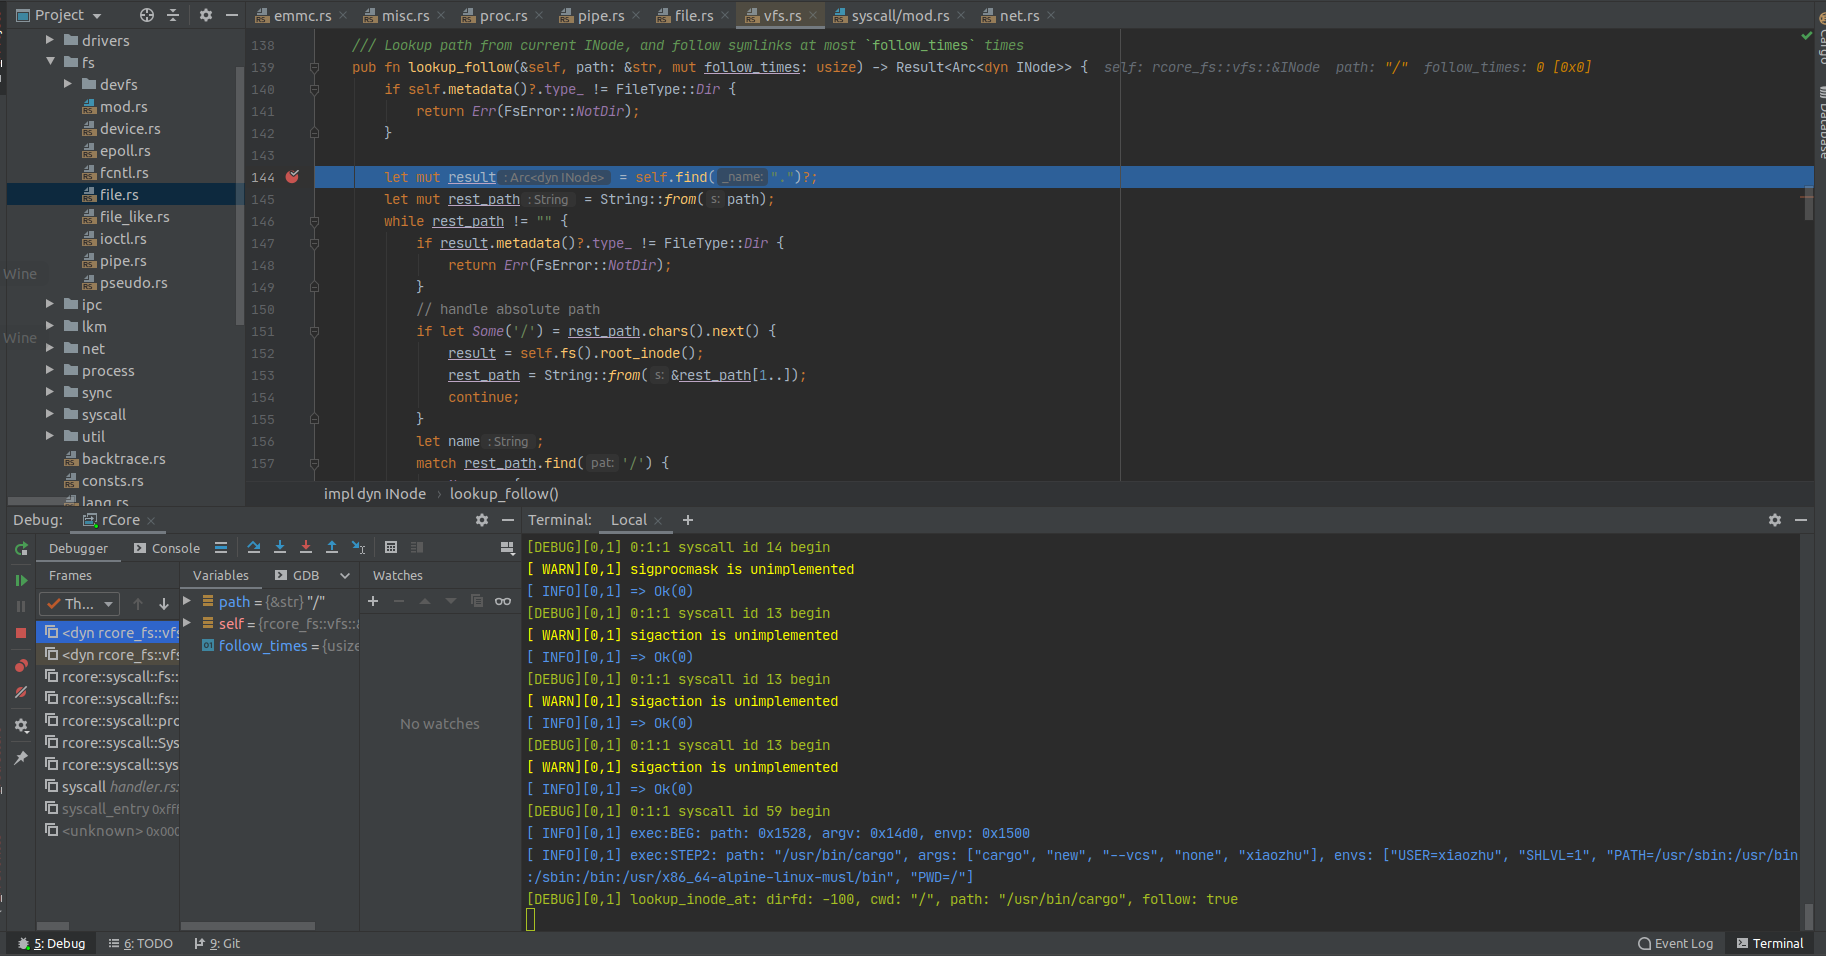
\includegraphics[width=\linewidth]{assets/gdb.png}
    \begin{figure}[]
        \centering
        
        % \caption{}
        % \label{}
    \end{figure}
\end{frame}

\begin{frame}{问题选讲}
    {IO 阻塞与进程死锁}
    \begin{itemize}
        \setlength{\itemsep}{10pt}
        \item 在有阻塞的 IO 中,目前的设计里 inode 的实现中看不见进程,
        并不能释放进程锁
        \item 于是,设想有如下情景:进程 2 由进程 1 fork 出来,并且有连接他们的管道,进程1读进程2写。
        进程1先读,保持着锁进入阻塞;进程2在写之前需要调用 getppid 获取父进程 id,便发生了死锁。
        \item 解决方法:考虑到进程的 pid 其实是定值,不必要用锁保护,可以和进程并列保存。
        \item 后续:IO 阻塞时释放进程锁
    \end{itemize}
\end{frame}

\begin{frame}{结束}
    谢谢观看
\end{frame}

\end{document}
